\documentclass[]{elsarticle} %review=doublespace preprint=single 5p=2 column
%%% Begin My package additions %%%%%%%%%%%%%%%%%%%
\usepackage[hyphens]{url}

  \journal{Journal of Memory and Language} % Sets Journal name


\usepackage{lineno} % add
\providecommand{\tightlist}{%
  \setlength{\itemsep}{0pt}\setlength{\parskip}{0pt}}

\usepackage{graphicx}
%%%%%%%%%%%%%%%% end my additions to header

\usepackage[T1]{fontenc}
\usepackage{lmodern}
\usepackage{amssymb,amsmath}
\usepackage{ifxetex,ifluatex}
\usepackage{fixltx2e} % provides \textsubscript
% use upquote if available, for straight quotes in verbatim environments
\IfFileExists{upquote.sty}{\usepackage{upquote}}{}
\ifnum 0\ifxetex 1\fi\ifluatex 1\fi=0 % if pdftex
  \usepackage[utf8]{inputenc}
\else % if luatex or xelatex
  \usepackage{fontspec}
  \ifxetex
    \usepackage{xltxtra,xunicode}
  \fi
  \defaultfontfeatures{Mapping=tex-text,Scale=MatchLowercase}
  \newcommand{\euro}{€}
\fi
% use microtype if available
\IfFileExists{microtype.sty}{\usepackage{microtype}}{}
\bibliographystyle{elsarticle-harv}
\usepackage{graphicx}
\ifxetex
  \usepackage[setpagesize=false, % page size defined by xetex
              unicode=false, % unicode breaks when used with xetex
              xetex]{hyperref}
\else
  \usepackage[unicode=true]{hyperref}
\fi
\hypersetup{breaklinks=true,
            bookmarks=true,
            pdfauthor={},
            pdftitle={Assessing replication rates in journals of experimental linguistics},
            colorlinks=false,
            urlcolor=blue,
            linkcolor=magenta,
            pdfborder={0 0 0}}
\urlstyle{same}  % don't use monospace font for urls

\setcounter{secnumdepth}{0}
% Pandoc toggle for numbering sections (defaults to be off)
\setcounter{secnumdepth}{0}

% Pandoc citation processing
\newlength{\cslhangindent}
\setlength{\cslhangindent}{1.5em}
\newlength{\csllabelwidth}
\setlength{\csllabelwidth}{3em}
% for Pandoc 2.8 to 2.10.1
\newenvironment{cslreferences}%
  {}%
  {\par}
% For Pandoc 2.11+
\newenvironment{CSLReferences}[2] % #1 hanging-ident, #2 entry spacing
 {% don't indent paragraphs
  \setlength{\parindent}{0pt}
  % turn on hanging indent if param 1 is 1
  \ifodd #1 \everypar{\setlength{\hangindent}{\cslhangindent}}\ignorespaces\fi
  % set entry spacing
  \ifnum #2 > 0
  \setlength{\parskip}{#2\baselineskip}
  \fi
 }%
 {}
\usepackage{calc}
\newcommand{\CSLBlock}[1]{#1\hfill\break}
\newcommand{\CSLLeftMargin}[1]{\parbox[t]{\csllabelwidth}{#1}}
\newcommand{\CSLRightInline}[1]{\parbox[t]{\linewidth - \csllabelwidth}{#1}\break}
\newcommand{\CSLIndent}[1]{\hspace{\cslhangindent}#1}

% Pandoc header



\begin{document}
\begin{frontmatter}

  \title{Assessing replication rates in journals of experimental
linguistics}
    \author[University of Osnabrück]{Kristina Kobrock\corref{1}}
   \ead{kkobrock@uni-osnabrueck.de} 
    \author[Universitetet i Oslo]{Timo B. Roettger}
  
      \address[University of Osnabrück]{Institute of Cognitive Science,
Wachsbleiche 27, 49090 Osnabrück}
    \address[Universitetet i Oslo]{Department of Linguistics and
Scandinavian Studies}
      \cortext[1]{Corresponding Author}
  
  \begin{abstract}
  This is the abstract. \textasciitilde150 words, avoid references,
  optional graphical abstract, keywords (max. 6, avoid abbreviations, AE
  spelling)

  It consists of two paragraphs.
  \end{abstract}
  
 \end{frontmatter}

\hypertarget{introduction}{%
\section{Introduction}\label{introduction}}

The replication of results is an integral part of cumulative
experimental science (e.g., Campbell, 1969; Rosenthal, 1990; Zwaan et
al., 2018). Yet, various scientific disciplines are currently facing
what is often referred to as the ``replication crisis,'' a state of
affairs that is characterized by an alarming amount of failed
replication attempts (Fidler and Wilcox, 2018). Here, we define
replications as studies that arrive at the same scientific conclusions
as an initial study, collecting new data and completing new analyses by
using the same methodology (see Barba, 2018 for a comprehensive overview
of different terminological uses). Coordinated efforts to replicate
published findings have uncovered surprisingly low rates of successful
replications in fields such as psychology (Open Science Collaboration,
2015), economics (Camerer et al., 2016) and social sciences (Camerer et
al., 2018). One driving factor of this lack of replicability is an
asymmetric incentive system that rewards novel confirmatory findings
over direct replications and null results. Replication studies are not
very popular because the necessary time and resource investment are not
appropriately rewarded in contemporary academic incentive systems (e.g.,
Koole and Lakens, 2012; Nosek et al., 2012). Both successful
replications (Madden et al., 1995) and repeated failures to replicate
(e.g., Doyen et al., 2012) are rarely published, and if they are
published they are usually published in less prestigious outlets than
the original findings. These dynamics lead to an abundance of positive
findings in the absence of possible conflicting negative evidence (see
also e.g. Fanelli, 2010).

Researchers from fields such as psychology (Makel et al., 2012),
education science (Makel and Plucker, 2014), and special education
research (Makel et al., 2016) have assessed the amount of direct
replications in their respective fields and report low replication rates
ranging from 0.13\% in the education sciences to 1.07\% in psychology
publications.

Experimental linguistics shares research practices that have been shown
to decrease the replicability of findings. Thus, there are raising
concerns about a similarly low number of replication studies conducted
and published in this field (e.g. Marsden et al., 2018; Roettger and
Baer-Henney, 2019). A number of failed replication attempts reported in
various subfields of linguistics indicate that these concerns are
warrented (e.g.~in language comprehension: Papesh, 2015; predictive
processing: Nieuwland et al., 2018; among others: Chen, 2007; Stack et
al., 2018; Westbury, 2018).

In order to thoroughly understand and be able to address this problem,
it is important to assess the number of replication attempts and their
contributing factors.

The present study assessed the frequency and typology of replication
studies that have been published in a representative sample of
experimental linguistic journals from 1988 to 2020. Our study aims at
answering two main questions: How many direct replications are published
in experimental linguistics? Are there factors that affect the
replication rates that are either found at the journal level
(e.g.~journal policies, open access, journal impact factor, etc.) or at
the study level (author composition, investigated language, etc.)

The study consisted of two analyses parts: First, we assessed the rate
of mentioning the term replication (search string: replic*) across 100
linguistic journals. Second, we categorized the type of replication
studies (direct, partial, conceptual) in a subset subset of twenty
journals. We then related their prevalence to factors like the year of
publication, and the citation and publication year of the initial study.

\hypertarget{how-often-do-journals-mention-the-term-replication}{%
\section{How often do journals mention the term
replication?}\label{how-often-do-journals-mention-the-term-replication}}

The key dependent variable of the first part of this study was the rate
of replication mention for journals relevant to the field of
experimental linguistics.

\hypertarget{material-and-methods}{%
\subsubsection{Material and methods}\label{material-and-methods}}

The study design has been preregistered at 2021-03-08 and can be
inspected \href{https://osf.io/9ceas/}{here: https://osf.io/9ceas/}. In
order to determine the rates of replication mention for individual
journals, we drew on a method introduced by Makel et al. (2012). First,
a sample of 100 journals relevant to the field of experimental
linguistics has been identified by making use of the search engine
\href{https://webofknowledge.com}{``Web of Science''
(https://webofknowledge.com)} at 2021-03-03. We restricted the search
results to journals in the web of science category ``Linguistics'' which
had at least 100 articles published and a high ratio of articles
containing the term ``experiment*'' in title, abstract or keywords . All
articles categorized as written in English between 1945-2020 were taken
into account. We selected a subset of those 100 journals that had the
highest ratio of mentioning the term ``experiment*.'' Two journals,
namely ``Language and Cognitive Processes'' and ``Language, Cognition
and Neuroscience'' had to be excluded because it turned out during
analysis that both journals have been renamed in 2013 and that these
have already been included in our sample.

The ratio between overall number of articles and those articles
mentioning the term ``experiment*'' ranged between 6.1 and 60.3 (with a
median of 11.5). The full list of journals can be inspected
\href{https://osf.io/q2e9k/}{here: https://osf.io/q2e9k/}. Albeit a
rough proxy, this procedure helped us identifying journals relevant to
the field of experimental linguistics. After journal selection, we
obtained the total number of articles containing the search term
``replicat*'' in title, abstract or keywords via Web of Science search.
Following the method used by Makel et al. (2012), the rates of
replication mention are calculated by dividing the number of articles
containing the term ``replicat*'' by the total number of articles for
each journal. As we were only interested in experimental linguistic
studies, we only included articles containing the search term
``experiment*'' in this formula.

Replication mentions are related to three journal properties: Journal
policies related to replication studies, journal impact factor and
whether the journal is open access or not. We examined the journals'
submission guidelines adopting a method suggested by Martin and Clarke
(2017). They grouped psychology journals into four categories dependent
on whether they (explicitly) encourage replication studies or not in
their ``instructions to authors'' and ``aims and scope'' sections on the
journal websites. For our analysis, we only distinguished between those
journals explicitly encouraging replication studies and those that do
not.

We extracted Journal Impact Factors via Journal Citation Reports
(https://jcr.clarivate.com).\footnote{The 2019 journal impact factors
  are calculated by dividing the citations in 2019 to items published in
  2017 and 2018 by the total number of citable items in 2017 and 2018.}

We assessed whether journals published open access via Web of Science.
We distinguished between three categories: journals which are listed in
the Directory of Open Access Journals (DOAJ) (``DOAJ gold''), journals
with some articles being published as open access articles (``partial'')
and journals with no option to publish open access (``no'').

\hypertarget{results}{%
\subsubsection{Results}\label{results}}

Out of the 51272 articles in our sample, 8006 mentioned the term
experiment* in title, abstract, or keywords. Out of these articles, 347
contained the term ``replic*.'' Thus 4.3\% of all experimental articles
in our sample mentioned the term ``replic*.''

The distribution of the mention rate substantially varies across
journals ranging from 0 to 1280\%. Overall, almost half of all journals
(n = 43) did not mention the term in any of their articles. The median
mention rate across journals is 1.6 (SD = 3.3). This mentioning rate is
comparable to the 1.6\% that Makel et al. (2012) have reported on in
their study on psychology. Figure X illustrated the variation across
those journals that exhibited at least one mention of the term.

\begin{center}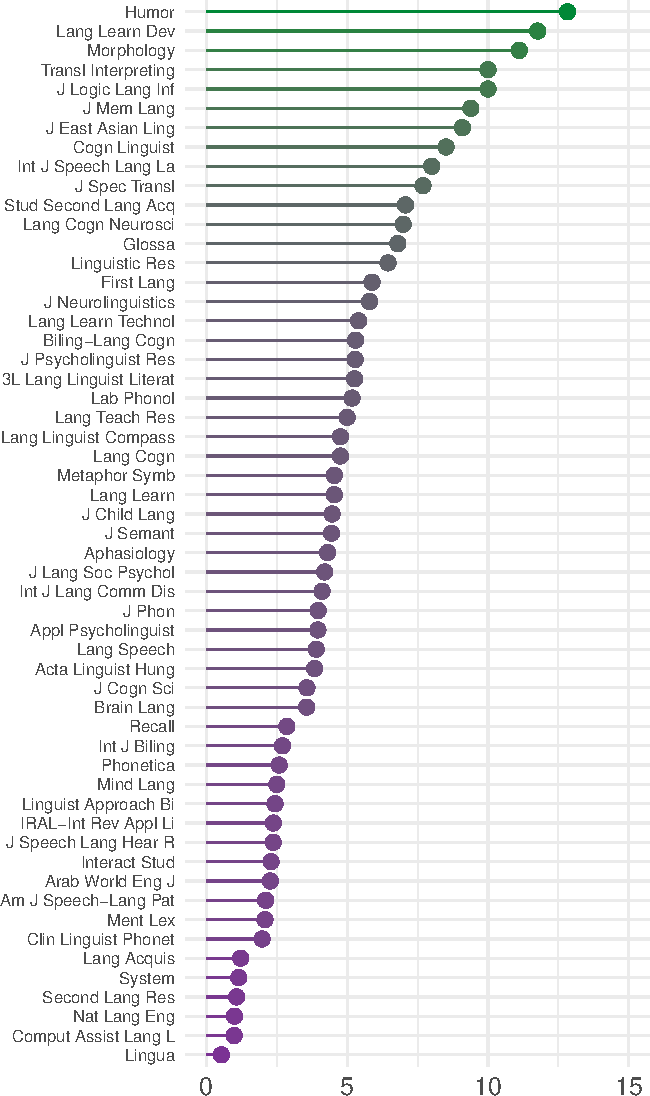
\includegraphics[width=1\linewidth]{ReplicationLing_files/figure-latex/topten_plot-1} \end{center}

Following preregistered protocol, we statistically estimated the mention
rate as predicted relative to the following factors: journal impact
factors (continuous), open access (binary: open access journal or not),
and replication policies (binary: either explicitly encourage or not).
We used Bayesian parameter estimation based on generalized linear
regression models with a binomial link function. The model was fitted to
the proportion of replication mentions per journal using the R package
brms (Bürkner, 2016). We used weakly informative normal priors centered
on 0 (sd = 2.5) for the intercept and Cauchy priors centered on zero
(scale = 2.5) for all population-level regression coefficients. These
priors are what is referred to as regularizing (Gelman et al., 2008),
i.e.~our prior assumption is agnostic as to whether the predictors
affect the dependent variable, thus making our model conservative with
regards to the predictors under investigation. Four sampling chains with
2000 iterations each have been run for each model, with a warm-up period
of 1000 iterations. For relevant predictor levels and contrasts between
predictor levels, we report the posterior probability for the rate of
replication mention. We summarize these distributions by reporting the
posterior mean and the 95\% credible intervals (calculated as the
highest posterior density interval).

The model estimates the proportion of replication mentions as 2.7\%
{[}1.7, 4.2{]} at a JIF of 0 and estimates an increase of the proportion
with each integer unit of JIF (log odds = 0.39 {[}0.29, 0.49{]}).
FigureX illustrates this relationship.

However, further explorations indicate that JIF is highly correlated
with the number of experimental studies reported in a journal (Spearman
correlation = 0.43). This correlation makes intuitively sense.
Experimental linguistic articles are often associated with psychology
adjacent fields, possibly attracting a broader audience and being cited
more widely. Given this correlation, it remains unclear if the term
``replicat*'' is used more often in high impact journals or simply more
common in journals that generally publish more experimental studies.

\begin{center}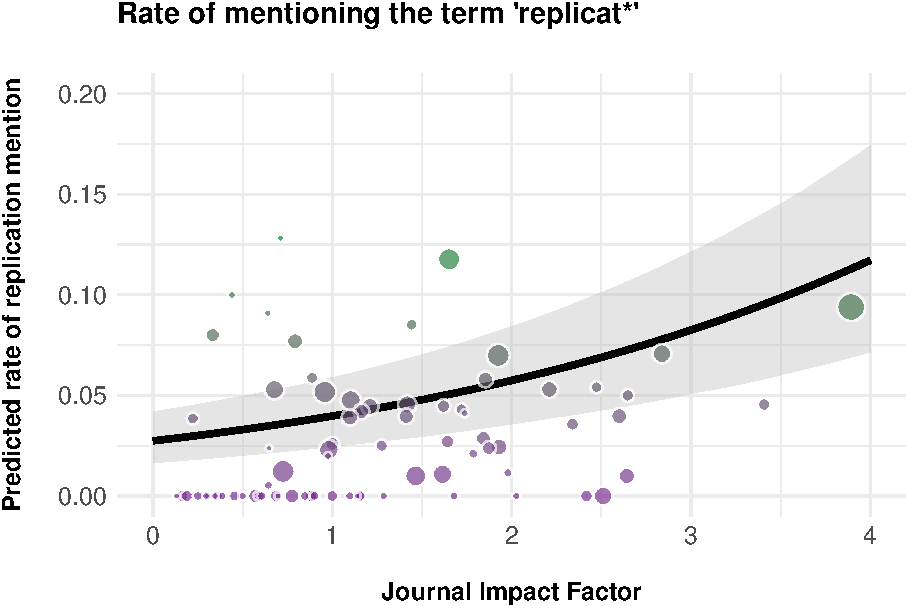
\includegraphics[width=1\linewidth]{ReplicationLing_files/figure-latex/plot_mention_jif-1} \end{center}

The model estimates the impact of whether the journal is open access or
not and whether replications are explicitly encouraged or not both as
positive, i.e.~the term replication is mentioned more often in both open
access journals and journals that explicitly encourage direct
replications. However, the uncertainty around these estimates is
substantial (open access: 0.41 {[}-0.41, 1.14{]}; policy: 0.24 {[}-0.27,
0.72{]}). The large amount of uncertainty surrounding the estimates is
not surprising given the small number of journals that explicitly
encourage direct replications (2 out of 98), and the small number of
open access journals (11 out of 98).

\hypertarget{how-many-of-these-mentions-are-actual-replications}{%
\section{How many of these mentions are actual
replications?}\label{how-many-of-these-mentions-are-actual-replications}}

The second part of the study aimed at obtaining a clearer picture about
what types of replication studies are published and whether direct
replications are becoming more frequent over time. Because the term
``replication'' is commonly used in ambiguous ways, the articles that
contained the search term ``replicat*'' required further analysis to
determine whether the articles in question indeed reported a replication
study or used the term in a different way.

\hypertarget{material-and-methods-1}{%
\subsubsection{Material and methods}\label{material-and-methods-1}}

From the superset of 100 journals obtained above, the first 20 journals
(i.e.~those journals with the highest proportion of experimental
studies) were selected for a more detailed analysis while excluding
journals for which less than 2 hits (TS=(replicat*)) could be obtained
(see \href{https://osf.io/f3yp8/}{here} for a list of article counts per
journal: https://osf.io/f3yp8/). Because of the skewed distribution of
our sample (114 hits for Journal of Memory and Language, and less than
40 for all other journals), we randomly selected 50 out of the 114
articles for the Journal of Memory and Language in order to achieve a
more balanced distribution of papers across journals (see
\href{https://osf.io/6vfpe/}{here} for details). The sampling procedure
above resulted in 210 possible self-labeled replication studies.

We identified whether the article in question indeed presented a
replication study or not. The relevant parts of the papers were title
and abstract of the paper, sentences around occurrences of the search
term ``replicat*'' as well as the paragraph before the Methods section
and the first paragraph of the Discussion section (following the
procedure specified by Makel et al. (2016)). If the authors explicitly
claimed that (one of) their research aim(s) was to replicate or methods
of an initial study, this article was treated as a replication and was
submitted to further analysis according to the preregistered coding
scheme \href{https://osf.io/ct2xj/}{here}: https://osf.io/ct2xj/.

When extracting number and types of changes made to the initial study,
we assumed that the authors of a replication study did not make any
drastic changes \emph{without} reporting them. The replication studies
were classified according to three types: direct replication (0
changes), partial replication (1 change) and conceptual replication (2
or more changes), following Marsden et al. (2018). We noted the nature
of the change as one of the following categories (yes/no): experimental
paradigm, sample, materials/experimental set-up, dependent variable,
independent variable, and control. We also noted the language under
investigation. The information on whether the article was published open
access as well as citation counts and years of publication for both
studies were obtained from Web of Science. An author overlap was
attested when at least one author was a (co-)author on both articles.

\hypertarget{results-1}{%
\subsubsection{Results}\label{results-1}}

Out of the 210 articles in the subsample, 117 were self-claimed
replications according to our criteria. The remaining 93 mentions were
xxx. Out of these replication studies, we categorized 66 as conceptual,
42 as partial, and only 8 as direct replications which amounts to 6.8\%
of all coded cases.

Looking closer at direct replications, 3 studies were independent
studies, i.e.~there was no overlap between authors of the initial study
and the replication study. Out of these independent direct replication
studies, 2 were self-labeled as successful replications. In other words,
our sample included only one independent failed replication attempt.

Figure X illustrates the development of replication studies across the
time span of our sample. While the overall number of studies increased
over the years, the proportion of direct replications remained stable at
best. However, it seems as if there is an increasing number of partial
and conceptual replications that was published within the last few
years.\footnote{Given the small number of direct replications in our
  sample, both a descriptive assessment and an inferential assessment as
  preregistered are very uninformative. The reader is directed to the
  supplementary materials, if they are interested in the model outputs
  of the preregistered analysis.}.

\begin{center}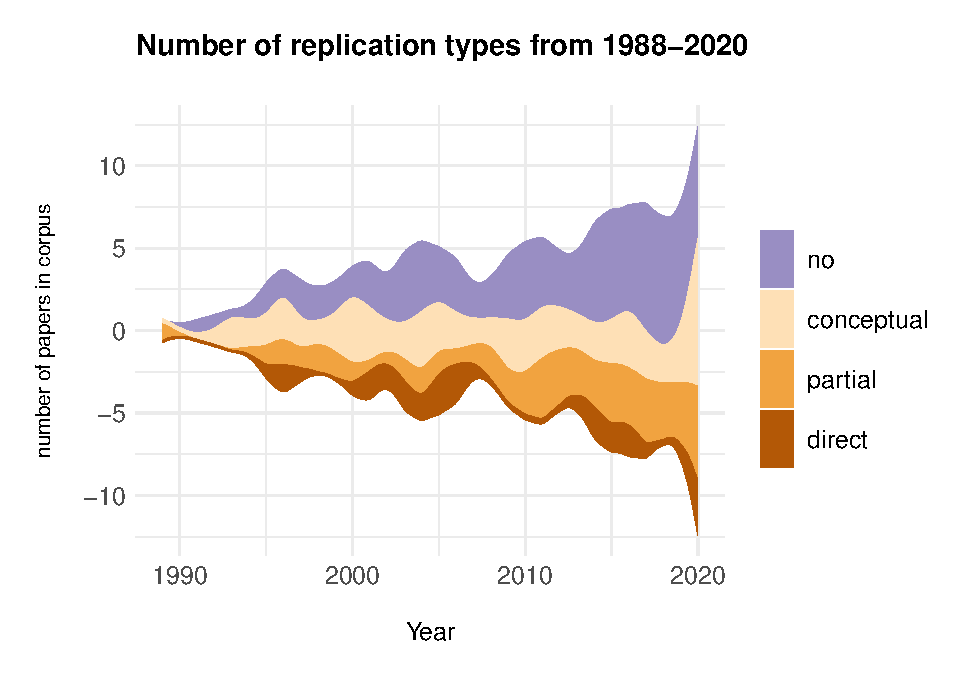
\includegraphics[width=1\linewidth]{ReplicationLing_files/figure-latex/steam_plot-1} \end{center}

One possible reason for the absence of increasing (direct) replication
rates could be that experimental linguistics predominantly replicates
experimental findings across languages, making it by definition at least
only a partial replication. However, only a minority of replications
targeted a different language than the initial study (15.4\%). The
majority of replication efforts were conducted within the same language
as the initial study. In fact, 66.7\% of all replication studies were
studies on English varieties.

The median number of years between an initial and a replication study is
7 years. Initial studies were on average 41.1 times cited before a
replication was published which amounts to a average yearly citation
rate of 5.9 citations. This is average citation rate was well above the
impact factor of journals in publishing experimental studies in
linguistics (median JIF in superset: 38). However, replications were on
average 17 times cited which amounts to only amounts to an average
yearly citation rate (calculated up to the time of analysis) of 0.6
citations. These numbers are in line with Marsden et al. (2018)
investigated the prevalence of replication studies across second
language research. They found that replication studies were on average
conducted after more than six years and over a hundred citations of the
original study. Thus, replications are either only performed after the
original study had already impacted the field substantially or is only
then published if the original study was impactful. The drop in
citations for replication studies compared to the initial study is in
line with the lack of perceived prestige of replication studies (e.g.,
Koole and Lakens, 2012; Nosek et al., 2012).

\hypertarget{case-study-of-journal-of-memory-and-language}{%
\subsubsection{Case study of Journal of Memory and
Language}\label{case-study-of-journal-of-memory-and-language}}

\begin{verbatim}
## type_replication
##            conceptual     direct    partial 
##       0.00       0.44       0.09       0.47
\end{verbatim}

\begin{verbatim}
##                 auth_overlap
## type_replication    0    1
##                  0.00 0.00
##       conceptual 0.18 0.26
##       direct     0.06 0.03
##       partial    0.24 0.24
\end{verbatim}

\begin{verbatim}
## [1] 0.04
\end{verbatim}

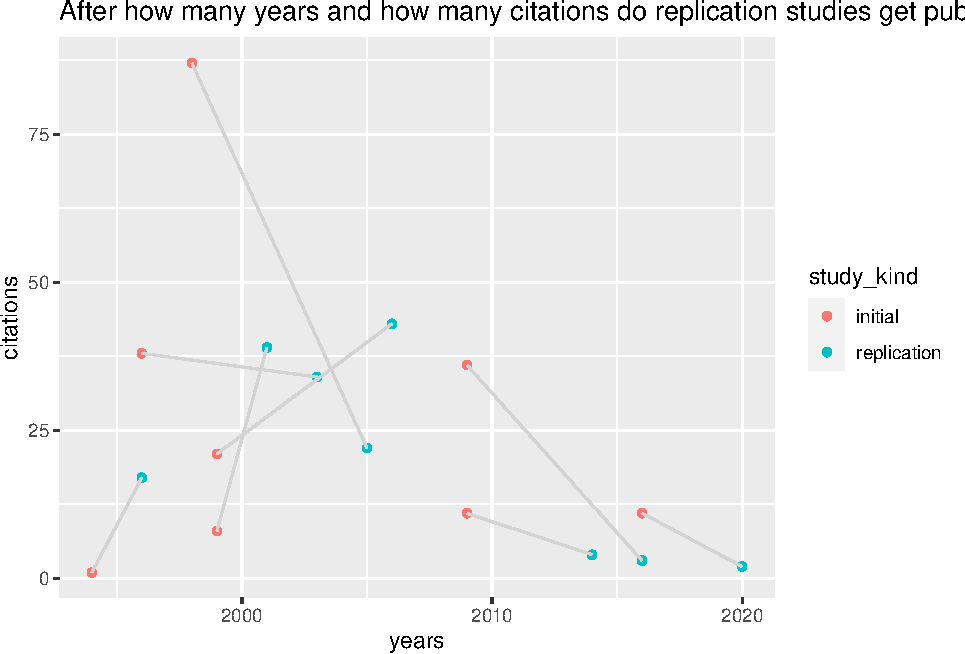
\includegraphics{ReplicationLing_files/figure-latex/plot cit and years direct-1.pdf}

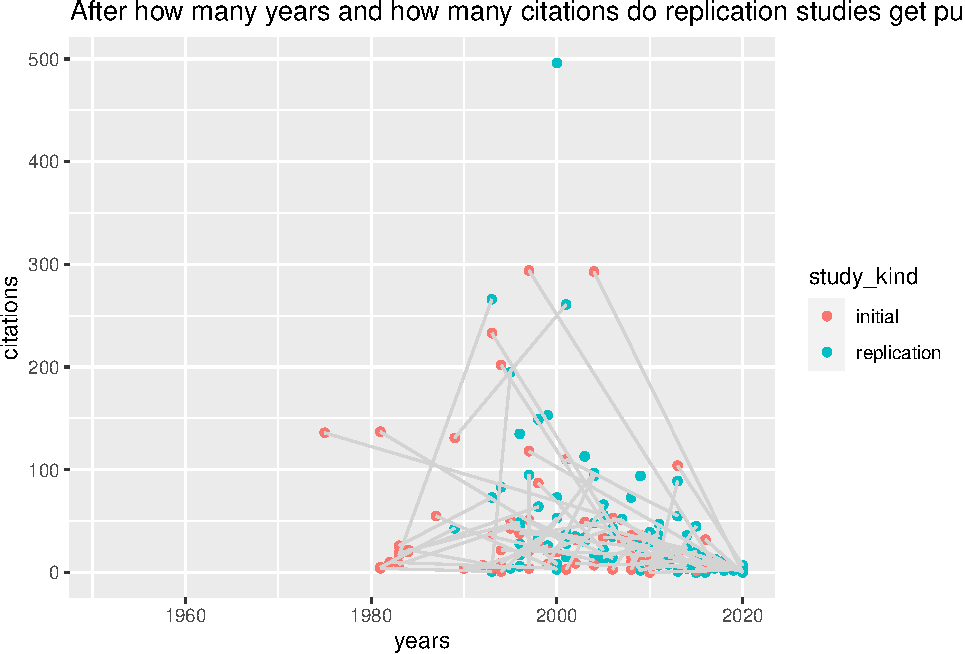
\includegraphics{ReplicationLing_files/figure-latex/plot cit and years all-1.pdf}

\hypertarget{discussion}{%
\subsubsection{Discussion}\label{discussion}}

\begin{itemize}
\tightlist
\item
  too little replication attempts in experimental linguistics
\item
  journals guidelines generally don't encourage replication studies
\item
  \ldots{}
\end{itemize}

\hypertarget{general-discussion}{%
\section{General discussion}\label{general-discussion}}

\begin{itemize}
\tightlist
\item
  compare rate of replication mention to previous studies in different
  fields --\textgreater{} broader picture
\end{itemize}

\hypertarget{caveats}{%
\subsubsection{Caveats}\label{caveats}}

This procedure is necessarily only a rough proxy of relevant
experimental linguistic articles published in the field and several
articles might thus have been overlooked and not been included in the
analysis.

\hypertarget{appendices}{%
\section{Appendices}\label{appendices}}

identified as A, B, etc.

\hypertarget{references}{%
\section*{References}\label{references}}
\addcontentsline{toc}{section}{References}

\hypertarget{refs}{}
\begin{CSLReferences}{1}{0}
\leavevmode\vadjust pre{\hypertarget{ref-barba_terminologies_2018}{}}%
Barba, L.A., 2018. Terminologies for {Reproducible} {Research}.

\leavevmode\vadjust pre{\hypertarget{ref-burkner_brms_2016}{}}%
Bürkner, P.-C., 2016. Brms: {An} {R} package for {Bayesian} multilevel
models using {Stan}. Journal of Statistical Software 80, 1--28.

\leavevmode\vadjust pre{\hypertarget{ref-camerer_evaluating_2016}{}}%
Camerer, C.F., Dreber, A., Forsell, E., Ho, T.-H., Huber, J.,
Johannesson, M., Kirchler, M., Almenberg, J., Altmejd, A., Chan, T.,
Heikensten, E., Holzmeister, F., Imai, T., Isaksson, S., Nave, G.,
Pfeiffer, T., Razen, M., Wu, H., 2016. Evaluating replicability of
laboratory experiments in economics. Science 351, 1433--1436.
doi:\href{https://doi.org/10.1126/science.aaf0918}{10.1126/science.aaf0918}

\leavevmode\vadjust pre{\hypertarget{ref-camerer_evaluating_2018}{}}%
Camerer, C.F., Dreber, A., Holzmeister, F., Ho, T.-H., Huber, J.,
Johanesson, M., Kirchler, M., Nave, G., Nosek, B.A., Pfeiffer, T.,
Altmejd, A., Buttrick, N., Chan, T., Chen, Y., Forsell, E., Gampa, A.,
Heikensten, E., Hummer, L., Imai, T., Isaksson, S., Manfredi, D., Rose,
J., Wagenmakers, E.-J., Wu, H., 2018. Evaluating the replicability of
social science experiments in {Nature} and {Science} between 2010 and
2015. Nature 2, 637--644.
doi:\href{https://doi.org/10.1038/s41562-018-0399-z}{10.1038/s41562-018-0399-z}

\leavevmode\vadjust pre{\hypertarget{ref-campbell_reforms_1969}{}}%
Campbell, D.T., 1969. Reforms as experiments. American Psychologist 24,
409.

\leavevmode\vadjust pre{\hypertarget{ref-chen_chinese_2007}{}}%
Chen, J.-Y., 2007. Do {Chinese} and {English} speakers think about time
differently? {Failure} of replicating {Boroditsky} (2001). Cognition
104, 427--436.

\leavevmode\vadjust pre{\hypertarget{ref-doyen_behavioral_2012}{}}%
Doyen, S., Klein, O., Pichon, C.-L., Cleeremans, A., 2012. Behavioral
priming: It's all in the mind, but whose mind? PloS one 7, e29081.

\leavevmode\vadjust pre{\hypertarget{ref-fanelli_pressures_2010}{}}%
Fanelli, D., 2010. Do pressures to publish increase scientists' bias? An
empirical support from US states data. PLoS ONE 5, e10271.
doi:\href{https://doi.org/10.1371/journal.pone.0010271}{10.1371/journal.pone.0010271}

\leavevmode\vadjust pre{\hypertarget{ref-fidler_reproducibility_2018}{}}%
Fidler, F., Wilcox, J., 2018. Reproducibility of scientific results.

\leavevmode\vadjust pre{\hypertarget{ref-gelman_weakly_2008}{}}%
Gelman, A., Jakulin, A., Pittau, M.G., Su, Y.-S., others, 2008. A weakly
informative default prior distribution for logistic and other regression
models. The Annals of Applied Statistics 2, 1360--1383.

\leavevmode\vadjust pre{\hypertarget{ref-koole_rewarding_2012}{}}%
Koole, S.L., Lakens, D., 2012. Rewarding replications: {A} sure and
simple way to improve psychological science. Perspectives on
Psychological Science 7, 608--614.

\leavevmode\vadjust pre{\hypertarget{ref-madden_how_1995}{}}%
Madden, C.S., Easley, R.W., Dunn, M.G., 1995. How journal editors view
replication research. Journal of Advertising 24, 77--87.

\leavevmode\vadjust pre{\hypertarget{ref-makel_facts_2014}{}}%
Makel, M.C., Plucker, J.A., 2014. Facts are more important than novelty:
{Replication} in the education sciences. Educational Researcher 43,
304--316.

\leavevmode\vadjust pre{\hypertarget{ref-makel_replication_2016}{}}%
Makel, M.C., Plucker, J.A., Freeman, J., Lombardi, A., Simonsen, B.,
Coyne, M., 2016. Replication of {Special} {Education} {Research}:
{Necessary} but {Far} {Too} {Rare}. Remedial and Special Education 37,
205--212.

\leavevmode\vadjust pre{\hypertarget{ref-makel_replications_2012}{}}%
Makel, M.C., Plucker, J.A., Hegarty, B., 2012. Replications in
psychology research: {How} often do they really occur? Perspectives on
Psychological Science 7, 537--542.

\leavevmode\vadjust pre{\hypertarget{ref-marsden_replication_2018}{}}%
Marsden, E., Morgan‐Short, K., Thompson, S., Abugaber, D., 2018.
Replication in {Second} {Language} {Research}: {Narrative} and
{Systematic} {Reviews} and {Recommendations} for the {Field}. Language
Learning 68, 321--391. doi:\href{https://doi.org/gc3h3b}{gc3h3b}

\leavevmode\vadjust pre{\hypertarget{ref-martin_are_2017}{}}%
Martin, G.N., Clarke, R.M., 2017. Are {Psychology} {Journals}
{Anti}-replication? {A} {Snapshot} of {Editorial} {Practices}. Frontiers
in Psychology 8.
doi:\href{https://doi.org/10.3389/fpsyg.2017.00523}{10.3389/fpsyg.2017.00523}

\leavevmode\vadjust pre{\hypertarget{ref-nieuwland_large-scale_2018}{}}%
Nieuwland, M.S., Politzer-Ahles, S., Heyselaar, E., Segaert, K., Darley,
E., Kazanina, N., Zu Wolfsthurn, S.V.G., Bartolozzi, F., Kogan, V., Ito,
A., Mézière, D., Barr, D.J., Rousselet, G.A., Ferguson, H.J.,
Bush-Moreno, S., Fu, X., Tuomainen, J., Kulakova, E., Husband, M.E.,
Donaldson, D.I., Kohút, Z., Rueschemeyer, S.-A., Huettig, F., 2018.
Large-scale replication study reveals a limit on probabilistic
prediction in language comprehension. eLife 7, e33468.
doi:\href{https://doi.org/10.7554/eLife.33468.001}{10.7554/eLife.33468.001}

\leavevmode\vadjust pre{\hypertarget{ref-nosek_scientific_2012}{}}%
Nosek, B.A., Spies, J.R., Motyl, M., 2012. Scientific utopia {II}.
{Restructuring} incentives and practices to promote truth over
publishability. Perspectives on Psychological Science 7, 615--631.

\leavevmode\vadjust pre{\hypertarget{ref-open_science_collaboration_estimating_2015}{}}%
Open Science Collaboration, 2015. Estimating the reproducibility of
psychological science. Science 349.
doi:\href{https://doi.org/10.1126/science.aac4716}{10.1126/science.aac4716}

\leavevmode\vadjust pre{\hypertarget{ref-papesh_just_2015}{}}%
Papesh, M.H., 2015. Just out of reach: {On} the reliability of the
action-sentence compatibility effect. Journal of Experimental
Psychology: General 144, e116--e141.
doi:\href{https://doi.org/10.1037/xge0000125}{10.1037/xge0000125}

\leavevmode\vadjust pre{\hypertarget{ref-roettger_toward_2019}{}}%
Roettger, T.B., Baer-Henney, D., 2019. Toward a replication culture:
{Speech} production research in the classroom. Phonological Data and
Analysis 1, 1--23.

\leavevmode\vadjust pre{\hypertarget{ref-rosenthal_replication_1990}{}}%
Rosenthal, R., 1990. Replication in behavioral research. Journal of
Social Behavior and Personality 5, 1.

\leavevmode\vadjust pre{\hypertarget{ref-stack_failure_2018}{}}%
Stack, C.M.H., James, A.N., Watson, D.G., 2018. A failure to replicate
rapid syntactic adaptation in comprehension. Memory \& Cognition 46,
864--877.
doi:\href{https://doi.org/10.3758/s13421-018-0808-6}{10.3758/s13421-018-0808-6}

\leavevmode\vadjust pre{\hypertarget{ref-westbury_implicit_2018}{}}%
Westbury, C., 2018. Implicit sound symbolism effect in lexical access,
revisited: {A} requiem for the interference task paradigm. Journal of
Articles in Support of the Null Hypothesis 15, 1--12.

\leavevmode\vadjust pre{\hypertarget{ref-zwaan_making_2018}{}}%
Zwaan, R.A., Etz, A., Lucas, R.E., Donnellan, M.B., 2018. Making
replication mainstream. Behavioral and Brain Sciences 41, E120.
doi:\href{https://doi.org/10.1017/S0140525X17001972}{10.1017/S0140525X17001972}

\end{CSLReferences}


\end{document}
